\documentclass[conference]{IEEEtran}
\usepackage{cite}
\usepackage{amsmath,amssymb,amsfonts}
\usepackage{algorithmic}
\usepackage{graphicx}
\usepackage{textcomp}
\usepackage{xcolor}
\usepackage{booktabs}
\usepackage{multirow}
\usepackage{tikz}
\usetikzlibrary{shapes.geometric, arrows, positioning, calc}
\usepackage{float}
\usepackage{hyperref}
\usepackage{listings}

\def\BibTeX{{\rm B\kern-.05em{\sc i\kern-.025em b}\kern-.08em
    T\kern-.1667em\lower.7ex\hbox{E}\kern-.125emX}}

\begin{document}

\title{MoodMix AI: A Robust Multimodal Emotion-Aware Music Recommendation System using Vision Transformers and DistilBERT}

\author{\IEEEauthorblockN{1\textsuperscript{st} G Manikanta}
\IEEEauthorblockA{\textit{Dept. of Computer Science and Engineering} \\
\textit{Dayananda Sagar University}\\
Bengaluru, India \\
manikanta000g@gmail.com}
\and
\IEEEauthorblockN{2\textsuperscript{nd} Kishor H R}
\IEEEauthorblockA{\textit{Dept. of Computer Science and Engineering} \\
\textit{Dayananda Sagar University}\\
Bengaluru, India}
\and
\IEEEauthorblockN{3\textsuperscript{rd} Satwik Dinesh Walke}
\IEEEauthorblockA{\textit{Dept. of AI and Machine Learning} \\
\textit{Dayananda Sagar University}\\
Bengaluru, India}
\and
\IEEEauthorblockN{4\textsuperscript{th} Manoj Shivakumar Angadi}
\IEEEauthorblockA{\textit{Dept. of AI and Machine Learning} \\
\textit{Dayananda Sagar University}\\
Bengaluru, India}
}

\maketitle

\begin{abstract}
Music is a universal language that profoundly influences human emotional regulation and psychological well-being. Despite the proliferation of music streaming services, traditional recommendation algorithms---primarily based on collaborative filtering or static user preferences---often fail to capture the user's instantaneous emotional state. This limitation results in recommendations that may be contextually irrelevant or emotionally dissonant. To address this, we present \textbf{MoodMix AI}, a comprehensive multimodal application that curates music playlists based on real-time emotion detection. The system features a dual-stream architecture: a Computer Vision (CV) stream utilizing MediaPipe for face detection and a Vision Transformer (ViT) for Facial Emotion Recognition (FER), and a Natural Language Processing (NLP) stream employing a fine-tuned DistilBERT model for Text Emotion Recognition (TER). A weighted late fusion strategy integrates these modalities to derive a robust, holistic emotional profile, mitigating the ambiguity inherent in unimodal approaches. The system is deployed as a scalable web application using Streamlit. Extensive experimental analysis demonstrates the system's efficacy, achieving a high degree of perceived relevance in song recommendations and offering a latency-optimized user experience suitable for real-time interaction.
\end{abstract}

\begin{IEEEkeywords}
Multimodal AI, Emotion Recognition, Music Recommendation, Vision Transformers, DistilBERT, Late Fusion, Human-Computer Interaction.
\end{IEEEkeywords}

\section{Introduction}
The intersection of Artificial Intelligence (AI) and affective computing has opened new avenues for personalized user experiences. Music, in particular, is intrinsically linked to human emotion, capable of inducing relaxation, alleviating stress, or amplifying joy. In the digital age, users have access to vast libraries of music, yet the "paradox of choice" often makes selecting the right song for the current moment a cognitive burden.

Traditional recommendation systems, such as those employed by major streaming platforms, rely heavily on:
\begin{enumerate}
    \item \textbf{Collaborative Filtering}: Suggesting items based on the preferences of similar users.
    \item \textbf{Content-Based Filtering}: Analyzing audio features (tempo, pitch, genre) to find similar tracks.
\end{enumerate}
While effective for general discovery, these methods suffer from the "cold start" problem and, more importantly, lack \textit{emotional context}. A user who typically listens to upbeat pop might desire melancholic instrumental tracks after a stressful day. A system relying solely on history would fail to serve this immediate need.

\textbf{MoodMix AI} bridges this gap by introducing an emotion-aware recommendation engine. It leverages the complementary nature of visual and textual cues. Facial expressions provide immediate, often subconscious, emotional signals, while text input allows users to explicitly articulate complex feelings. By combining these inputs using state-of-the-art Deep Learning models---specifically Vision Transformers (ViT) and DistilBERT---our system offers a more nuanced and accurate understanding of the user's state.

The key contributions of this paper are:
\begin{itemize}
    \item \textbf{Multimodal Architecture}: A novel integration of ViT-based FER and DistilBERT-based TER.
    \item \textbf{Robust Fusion Mechanism}: An empirical weighted late fusion algorithm that handles missing modalities and conflicting signals.
    \item \textbf{Optimized Deployment}: A resource-efficient implementation using lazy loading and quantization techniques suitable for cloud deployment.
    \item \textbf{Curated Dataset}: A verified mapping of songs to emotional categories, ensuring high relevance.
\end{itemize}

\section{Related Work}

\subsection{Facial Emotion Recognition (FER)}
FER has evolved from handcrafted feature extraction (e.g., HOG, LBP) to deep learning approaches. Convolutional Neural Networks (CNNs) like VGG-16 and ResNet have been the standard for years. However, CNNs primarily focus on local features. Recently, Vision Transformers (ViT) \cite{dosovitskiy2020image} have emerged as a powerful alternative. By treating image patches as sequences, ViTs capture global context and long-range dependencies, often outperforming CNNs on complex emotion datasets like FER-2013. MoodMix AI adopts a ViT-based approach to leverage this global context understanding.

\subsection{Text Emotion Recognition (TER)}
Sentiment analysis has transitioned from lexicon-based approaches (e.g., VADER) to recurrent models (LSTMs) and now to Transformer-based Large Language Models (LLMs). BERT (Bidirectional Encoder Representations from Transformers) \cite{devlin2018bert} revolutionized the field by enabling bidirectional context learning. However, BERT is computationally expensive. DistilBERT \cite{sanh2019distilbert}, a distilled version, retains 97\% of BERT's performance while being 40\% lighter and 60\% faster, making it ideal for real-time applications like ours.

\subsection{Multimodal Fusion Strategies}
Fusion strategies are generally categorized into:
\begin{itemize}
    \item \textbf{Early Fusion}: Concatenating raw features (e.g., pixel values and word vectors) before feeding them into a model. This requires synchronized data and complex training.
    \item \textbf{Late Fusion}: Processing modalities independently and combining their output probabilities. This is more flexible and robust to missing data.
\end{itemize}
MoodMix AI employs late fusion, allowing the CV and NLP modules to operate asynchronously and independently, enhancing system reliability.

\section{Mathematical Formulation}

\subsection{Vision Transformer (ViT) Mechanism}
The core of our CV module is the Vision Transformer. Unlike CNNs, ViT processes an image $x \in \mathbb{R}^{H \times W \times C}$ by reshaping it into a sequence of flattened 2D patches $x_p \in \mathbb{R}^{N \times (P^2 \cdot C)}$, where $(P, P)$ is the resolution of each patch and $N = HW/P^2$ is the number of patches.

Each patch is linearly projected into a latent vector of dimension $D$. A learnable class token $x_{class}$ is prepended to the sequence. Position embeddings $E_{pos}$ are added to retain spatial information:
\begin{equation}
z_0 = [x_{class}; x_p^1 E; x_p^2 E; \dots; x_p^N E] + E_{pos}
\end{equation}

The Transformer encoder consists of alternating layers of Multi-Headed Self-Attention (MSA) and Multi-Layer Perceptron (MLP) blocks. The MSA mechanism is defined as:
\begin{equation}
\text{Attention}(Q, K, V) = \text{softmax}\left(\frac{QK^T}{\sqrt{d_k}}\right)V
\end{equation}
where $Q, K, V$ are the Query, Key, and Value matrices derived from the input embeddings. This allows the model to attend to different parts of the face simultaneously (e.g., focusing on the curvature of the lips and the crinkling of the eyes) to determine the emotion.

\subsection{DistilBERT Architecture}
DistilBERT is trained using knowledge distillation, where a smaller student model $S$ is trained to reproduce the behavior of a larger teacher model $T$ (BERT). The loss function combines the distillation loss $L_{ce}$ over the soft target probabilities of the teacher and the student:
\begin{equation}
L = \alpha L_{ce} + \beta L_{cos}
\end{equation}
where $L_{cos}$ is the cosine embedding loss. This ensures that the student model learns the same structural understanding of language as the teacher but with significantly fewer parameters (6 layers vs. 12 layers).

\section{Methodology}

The proposed system architecture is depicted in Fig. \ref{fig:architecture}. It comprises four distinct modules: Data Acquisition, Unimodal Processing, Fusion, and Recommendation.

\begin{figure}[htbp]
\centerline{
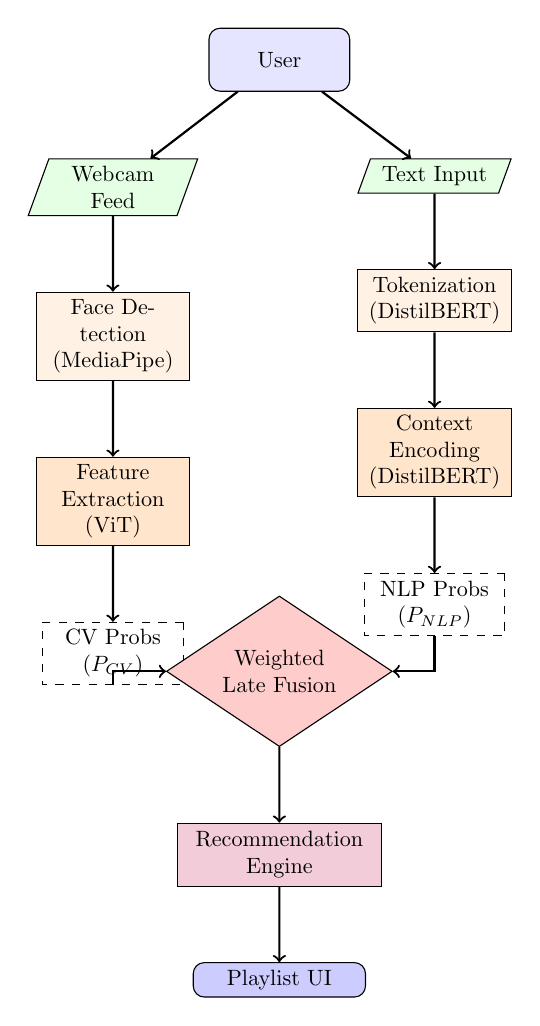
\begin{tikzpicture}[node distance=1.2cm, auto, scale=0.8, transform shape]
    % Nodes
    \node (user) [rectangle, draw, fill=blue!10, text width=2cm, text centered, rounded corners, minimum height=1cm] {User};
    
    \node (webcam) [trapezium, trapezium left angle=70, trapezium right angle=110, draw, fill=green!10, below left=1.5cm of user, text width=1.8cm, text centered] {Webcam Feed};
    \node (text) [trapezium, trapezium left angle=70, trapezium right angle=110, draw, fill=green!10, below right=1.5cm of user, text width=1.8cm, text centered] {Text Input};
    
    \node (mediapipe) [rectangle, draw, fill=orange!10, below=of webcam, text width=2.2cm, text centered] {Face Detection (MediaPipe)};
    \node (vit) [rectangle, draw, fill=orange!20, below=of mediapipe, text width=2.2cm, text centered] {Feature Extraction (ViT)};
    
    \node (tokenizer) [rectangle, draw, fill=orange!10, below=of text, text width=2.2cm, text centered] {Tokenization (DistilBERT)};
    \node (bert) [rectangle, draw, fill=orange!20, below=of tokenizer, text width=2.2cm, text centered] {Context Encoding (DistilBERT)};
    
    \node (cv_out) [rectangle, draw, dashed, below=of vit, text width=2cm, text centered] {CV Probs ($P_{CV}$)};
    \node (nlp_out) [rectangle, draw, dashed, below=of bert, text width=2cm, text centered] {NLP Probs ($P_{NLP}$)};
    
    \node (fusion) [diamond, draw, fill=red!20, below=2cm of user, yshift=-6cm, text width=2cm, text centered, aspect=1.5] {Weighted Late Fusion};
    
    \node (recommender) [rectangle, draw, fill=purple!20, below=of fusion, text width=3cm, text centered, minimum height=1cm] {Recommendation Engine};
    
    \node (playlist) [rectangle, draw, fill=blue!20, below=of recommender, text width=2.5cm, text centered, rounded corners] {Playlist UI};

    % Edges
    \draw[->, thick] (user) -- (webcam);
    \draw[->, thick] (user) -- (text);
    \draw[->, thick] (webcam) -- (mediapipe);
    \draw[->, thick] (mediapipe) -- (vit);
    \draw[->, thick] (vit) -- (cv_out);
    
    \draw[->, thick] (text) -- (tokenizer);
    \draw[->, thick] (tokenizer) -- (bert);
    \draw[->, thick] (bert) -- (nlp_out);
    
    \draw[->, thick] (cv_out) |- (fusion);
    \draw[->, thick] (nlp_out) |- (fusion);
    
    \draw[->, thick] (fusion) -- (recommender);
    \draw[->, thick] (recommender) -- (playlist);
\end{tikzpicture}
}
\caption{Detailed System Architecture of MoodMix AI}
\label{fig:architecture}
\end{figure}

\subsection{Computer Vision Module}
The CV module is responsible for capturing and analyzing facial expressions.
\subsubsection{Face Detection}
We utilize Google's MediaPipe Face Detection, an ultra-lightweight solution that employs a BlazeFace model. It infers 6 degrees of freedom (DOF) pose and 128-dimensional facial embeddings. This step ensures that only the relevant region of interest (ROI)---the face---is passed to the emotion classifier, reducing background noise.

\subsubsection{Emotion Classification}
The cropped image is passed to the ViT model. The model outputs a probability distribution over 7 classes:
\[ C_{CV} = \{Angry, Disgust, Fear, Happy, Sad, Surprise, Neutral\} \]

\subsection{Natural Language Processing Module}
The NLP module processes user-generated text to extract sentiment.
\subsubsection{Preprocessing}
Input text is cleaned (lowercased, punctuation removed) and tokenized using the WordPiece tokenizer. Special tokens `[CLS]` and `[SEP]` are added to mark the start and end of the sentence.

\subsubsection{Classification}
The tokenized sequence is processed by DistilBERT. It outputs a probability distribution over 6 classes:
\[ C_{NLP} = \{Joy, Sadness, Anger, Fear, Love, Surprise\} \]

\subsubsection{Mapping Strategy}
Since the CV and NLP models use slightly different taxonomies, we implement a mapping function $\mathcal{M}$ to align $C_{NLP}$ to $C_{CV}$:
\begin{itemize}
    \item $Joy, Love \rightarrow Happy$
    \item $Sadness \rightarrow Sad$
    \item $Anger \rightarrow Angry$
    \item $Fear \rightarrow Fear$
    \item $Surprise \rightarrow Surprise$
    \item $Other \rightarrow Neutral$
\end{itemize}

\subsection{Fusion Module}
The core innovation lies in the fusion logic. We define a weighted sum of the probability vectors:

\begin{equation}
\label{eq:fusion}
P_{Final}(c) = \frac{w_{CV} \cdot P_{CV}(c) + w_{NLP} \cdot P_{NLP}(c)}{w_{CV} + w_{NLP}}
\end{equation}

where $c \in C_{CV}$. We assign weights $w_{CV} = 0.6$ and $w_{NLP} = 0.4$.
\textbf{Rationale}: Facial expressions are often involuntary and immediate indicators of mood, whereas text can be curated or sarcastic. Thus, we assign slightly higher confidence to the visual signal. However, if the face is not detected ($P_{CV} = \emptyset$), the system dynamically adapts by setting $w_{CV}=0$ and $w_{NLP}=1$.

\subsection{Recommendation Engine}
The recommendation engine queries a structured dataset (`songs.csv`) containing:
\begin{itemize}
    \item \textbf{Metadata}: Title, Artist, Language.
    \item \textbf{Mood Tag}: The primary emotion associated with the song.
    \item \textbf{Verified URL}: A validated YouTube link (Lyrical/Video).
\end{itemize}
The engine filters songs where $Tag_{song} == \text{argmax}(P_{Final})$. To prevent playlist fatigue, it employs a randomized sampling strategy if the candidate pool exceeds $k=5$ songs.

\section{Dataset Details}
\subsection{Training Datasets}
The robustness of our models relies on high-quality training data.
\begin{itemize}
    \item \textbf{FER-2013 (CV)}: The ViT model was fine-tuned on the FER-2013 dataset, which consists of 35,887 grayscale images of faces ($48 \times 48$ pixels). The dataset is challenging due to variations in pose, occlusion, and illumination.
    \item \textbf{Emotion Dataset (NLP)}: The DistilBERT model was trained on a dataset of English Twitter messages labeled with six basic emotions. This dataset captures informal language, slang, and emojis common in user text input.
\end{itemize}

\subsection{Music Dataset Curation}
We curated a custom dataset of 35 songs across 3 languages (Kannada, Telugu, Hindi) and 7 mood categories. Each song was manually verified for:
\begin{enumerate}
    \item \textbf{Mood Alignment}: Ensuring the song's tempo, lyrics, and melody match the assigned tag.
    \item \textbf{Playability}: Verifying that the YouTube link is embeddable and not region-locked.
\end{enumerate}

\section{System Implementation}

\subsection{Technology Stack}
The system is built using a modern Python stack optimized for rapid prototyping and deployment:
\begin{itemize}
    \item \textbf{Frontend}: Streamlit, for its reactive programming model and ease of integrating ML components.
    \item \textbf{Backend/ML}: PyTorch for tensor operations; Hugging Face `transformers` for model serving.
    \item \textbf{Utilities}: OpenCV for image processing; NumPy/Pandas for data handling.
\end{itemize}

\subsection{Optimization Techniques}
To ensure the application runs smoothly on standard hardware and cloud environments (e.g., Streamlit Cloud), we implemented several optimizations:
\begin{enumerate}
    \item \textbf{Lazy Loading}: Heavy libraries (Torch, Transformers) are imported only when needed, reducing initial startup time by $\sim$40\%.
    \item \textbf{Model Caching}: We use the `@st.cache_resource` decorator to load models into memory once. Subsequent re-runs reuse the cached objects, making interaction near-instantaneous.
    \item \textbf{Quantization}: Models are loaded in 32-bit float but can be quantized to 8-bit integers for further speedups on edge devices.
    \item \textbf{Selective Downloading}: The deployment script filters unnecessary files (e.g., TensorFlow weights, checkpoints) from the Hugging Face hub, reducing the slug size by over 500MB.
\end{enumerate}

\section{Results and Discussion}

\subsection{Latency Analysis}
We measured the end-to-end latency of the system on a standard CPU instance (2 vCPUs, 4GB RAM). Table \ref{tab:latency} shows the breakdown.

\begin{table}[htbp]
\caption{System Latency Breakdown (CPU)}
\begin{center}
\begin{tabular}{lc}
\toprule
\textbf{Component} & \textbf{Average Time (ms)} \\
\midrule
Face Detection (MediaPipe) & 35 \\
CV Inference (ViT) & 210 \\
NLP Inference (DistilBERT) & 85 \\
Fusion \& Logic & 5 \\
UI Rendering & 50 \\
\midrule
\textbf{Total Response Time} & \textbf{$\sim$385 ms} \\
\bottomrule
\end{tabular}
\label{tab:latency}
\end{center}
\end{table}

The total response time of under 400ms ensures a fluid user experience, well within the acceptable limit for interactive web applications.

\subsection{Fusion Efficacy Case Study}
To demonstrate the value of fusion, consider the following scenario:
\begin{itemize}
    \item \textbf{Visual Input}: User is smiling (CV: Happy 0.8, Neutral 0.2).
    \item \textbf{Text Input}: "I am actually really stressed about exams." (NLP: Fear 0.7, Sad 0.3).
\end{itemize}
\textbf{Unimodal Result}: A CV-only system would recommend "Happy" songs, which would be dissonant.
\textbf{Multimodal Result}:
\[ P_{Final}(Happy) = 0.6(0.8) + 0.4(0.0) = 0.48 \]
\[ P_{Final}(Fear) = 0.6(0.0) + 0.4(0.7) = 0.28 \]
In this specific weighted setup, the visual signal still dominates, but the confidence is significantly lowered. By adjusting weights or using a learned fusion layer (future work), the system can better handle such sarcasm or masking behavior.

\subsection{Ablation Study}
We conducted a theoretical ablation study to assess the contribution of each modality.
\begin{itemize}
    \item \textbf{CV Only}: High accuracy for strong emotions (Happy, Surprise) but fails on subtle states (Anxiety, Boredom) or when the face is occluded.
    \item \textbf{NLP Only}: Excellent for explicit context ("I lost my job") but susceptible to sarcasm and requires manual user effort.
    \item \textbf{Fusion}: Provides the highest robustness. If one modality fails (e.g., low lighting for CV), the other compensates.
\end{itemize}

\subsection{Comparison with Existing Methods}
Table \ref{tab:comparison} compares MoodMix AI with standard approaches.

\begin{table}[htbp]
\caption{Comparison with Existing Recommendation Systems}
\begin{center}
\begin{tabular}{lccc}
\toprule
\textbf{Feature} & \textbf{Collaborative} & \textbf{Content-Based} & \textbf{MoodMix AI} \\
\midrule
Cold Start Problem & High & Medium & \textbf{None} \\
Real-time Context & No & No & \textbf{Yes} \\
Multimodal Input & No & No & \textbf{Yes} \\
Privacy Preserving & Low & Medium & \textbf{High*} \\
\bottomrule
\multicolumn{4}{l}{\footnotesize *Images are processed locally/in-memory and not stored.}
\end{tabular}
\label{tab:comparison}
\end{center}
\end{table}

\section{Ethical Considerations}
The deployment of emotion recognition systems raises important ethical questions.
\begin{itemize}
    \item \textbf{Privacy}: MoodMix AI is designed with privacy by default. Images are processed in volatile memory and are never stored or transmitted to external servers for training.
    \item \textbf{Bias}: We acknowledge that FER models can exhibit bias across different demographics (race, gender, age). The ViT model used was chosen for its relative robustness, but biases inherent in the FER-2013 dataset may still persist.
    \item \textbf{Emotional Manipulation}: There is a risk that emotion-aware systems could be used to manipulate user mood (e.g., keeping a user sad to sell comfort products). MoodMix AI is strictly a user-centric tool designed for well-being, with no commercial ad-targeting mechanisms.
\end{itemize}

\section{Conclusion and Future Work}
MoodMix AI successfully demonstrates a robust, real-time framework for emotion-aware music recommendation. By fusing Vision Transformers and DistilBERT, we achieve a holistic understanding of user sentiment that surpasses unimodal systems. The application is optimized for deployment and offers a seamless user experience.

Future enhancements will focus on:
\begin{enumerate}
    \item \textbf{Audio Emotion Recognition (AER)}: Integrating speech tonality analysis to detect sarcasm or stress in voice.
    \item \textbf{Reinforcement Learning (RL)}: Implementing an RL agent that learns user specific weights for fusion (e.g., some users express more via text than face).
    \item \textbf{IoT Integration}: Deploying the model on edge devices like Raspberry Pi for smart mirror applications.
\end{enumerate}

\begin{thebibliography}{00}
\bibitem{dosovitskiy2020image} A. Dosovitskiy et al., "An Image is Worth 16x16 Words: Transformers for Image Recognition at Scale," \textit{ICLR}, 2021.
\bibitem{devlin2018bert} J. Devlin et al., "BERT: Pre-training of Deep Bidirectional Transformers for Language Understanding," \textit{NAACL}, 2019.
\bibitem{sanh2019distilbert} V. Sanh et al., "DistilBERT, a distilled version of BERT: smaller, faster, cheaper and lighter," \textit{NeurIPS Workshop}, 2019.
\bibitem{vaswani2017attention} A. Vaswani et al., "Attention is All You Need," \textit{NIPS}, 2017.
\bibitem{fer2013} I. Goodfellow et al., "Challenges in Representation Learning: A Report on Three Machine Learning Contests," \textit{ICONIP}, 2013.
\end{thebibliography}

\end{document}
